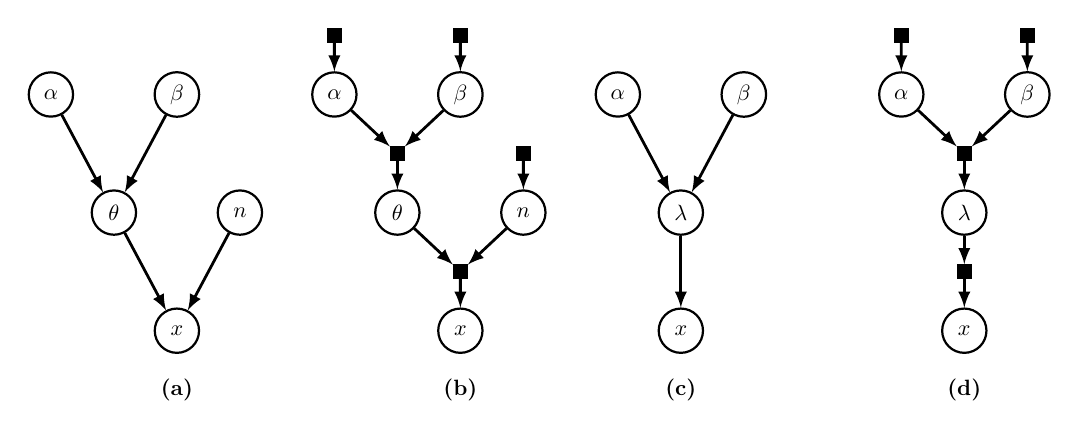
\begin{tikzpicture}[thick,xscale=0.8, yscale=.75, every node/.style={scale=0.8}]
\tikzset{vertex/.style = {shape=circle,draw,minimum size=2em}}
\tikzset{edge/.style = {->,> = latex, line width=1}}

% binomial beta directed graph
\begin{scope}
% vertices
\node[vertex] (a) at  (-1,2) {$\alpha$};
\node[vertex] (b) at  (1,2) {$\beta$};
\node[vertex] (x) at  (1, -2) {$x$};
\node[vertex] (n) at (2,0) {$n$};
\node[vertex] (t) at (0,0) {$\theta$};
%edges
\draw[edge] (a) to (t);
\draw[edge] (b) to (t);
\draw[edge] (t) to (x);
\draw[edge] (n) to (x);
\node at (1, -3) {\textbf{(a)}}; 
\end{scope}

% binomial beta factor graph
\begin{scope}[shift={(4.5,0)}]
% vertices
\node[vertex] (a) at  (-1,2) {$\alpha$};
\node[vertex] (b) at  (1,2) {$\beta$};
\node[vertex] (x) at  (1, -2) {$x$};
\node[vertex] (n) at (2,0) {$n$};
\node[vertex] (t) at (0,0) {$\theta$};
\begin{scope}[vertex/.style = {shape=rectangle, draw,minimum size=.1em, inner sep=3pt, fill=black}]
\node[vertex] (fone) at  (-1,3) {};
\node[vertex] (ftwo) at  (1,3) {};
\node[vertex] (fthree) at (0,1) {};
\node[vertex] (ffour) at (1,-1) {};
\node[vertex] (ffife) at (2,1) {};
\end{scope}
%edges

\draw[edge] (fone) to (a);
\draw[edge] (ftwo) to (b);
\draw[edge] (a) to (fthree);
\draw[edge] (b) to (fthree);
\draw[edge] (fthree) to (t);
\draw[edge] (t) to (ffour);
\draw[edge] (n) to (ffour);
\draw[edge] (ffour) to (x);
\draw[edge] (ffife) to (n);
\node at (1, -3) {\textbf{(b)}}; 
\end{scope}

% poisson gamma directed graph
\begin{scope}[shift={(9,0)}]
% vertices
\node[vertex] (a) at  (-1,2) {$\alpha$};
\node[vertex] (b) at  (1,2) {$\beta$};
\node[vertex] (l) at (0,0) {$\lambda$};
\node[vertex] (x) at (0,-2) {$x$};
%edges
\draw[edge] (a) to (l);
\draw[edge] (b) to (l);
\draw[edge] (l) to (x);
\node at (0, -3) {\textbf{(c)}}; 
\end{scope}

% poisson gamma factor graph
\begin{scope}[shift={(13.5,0)}]
% vertices
\node[vertex] (a) at  (-1,2) {$\alpha$};
\node[vertex] (b) at  (1,2) {$\beta$};
\node[vertex] (l) at (0,0) {$\lambda$};
\node[vertex] (x) at (0,-2) {$x$};
\begin{scope}[vertex/.style = {shape=rectangle, draw,minimum size=.1em, inner sep=3pt, fill=black}]
\node[vertex] (f1) at  (-1,3) {};
\node[vertex] (f2) at  (1,3) {};
\node[vertex] (f3) at  (0,1) {};
\node[vertex] (f4) at  (0,-1) {};
\end{scope}
%edges
\draw[edge] (f1) to (a);
\draw[edge] (f2) to (b);
\draw[edge] (a) to (f3);
\draw[edge] (b) to (f3);
\draw[edge] (f3) to (l);
\draw[edge] (l) to (f4);
\draw[edge] (f4) to (x);
\node at (0, -3) {\textbf{(d)}}; 
\end{scope}

\end{tikzpicture}

